\documentclass[conference]{IEEEtran}
\IEEEoverridecommandlockouts

\usepackage{cite}
\usepackage{amsmath,amssymb,amsfonts}
\usepackage{algorithmic}
\usepackage{graphicx}
\usepackage{textcomp}
\usepackage{xcolor}
\def\BibTeX{{\rm B\kern-.05em{\sc i\kern-.025em b}\kern-.08em
    T\kern-.1667em\lower.7ex\hbox{E}\kern-.125emX}}
\begin{document}

\title{Leveraging Deep Learning Techniques in
Skin Cancer Detection\\
}

\author{\IEEEauthorblockN{\textsuperscript{} Mundhir AL Bohri }
\IEEEauthorblockA{\textit{Dalhousie University} \\
\textit{Faculty of Computer Science}\\
\textit{
CSCI 4155 Machine Learning}\\
n409130@dal.ca}
\and
\IEEEauthorblockN{\textsuperscript{} Noof Al Shehhi }
\IEEEauthorblockA{\textit{Dalhousie University} \\
\textit{Faculty of Computer Science}\\
\textit{
CSCI 4155 Machine Learning}\\
noof.alshehhi@dal.ca}
\and
\IEEEauthorblockN{\textsuperscript{} Harsahib Preet Singh}
\IEEEauthorblockA{\textit{Dalhousie University} \\
\textit{Faculty of Computer Science}\\
\textit{
CSCI 4155 Machine Learning}\\
hr644654@dal.ca}
}

\maketitle

\begin{abstract}
In this project presents different approaches to skin cancer detection using deep learning. Recognizing skin cancer as a major health concern, the project leverages the capabilities of Convolutional Neural Networks (CNNs) to classify and detect various types of skin cancer. Utilizing the Skin Cancer MNIST: HAM10000 dataset [2], the team aims to develop a machine learning model that is both accurate and suitable for medical use. The project focuses on data preprocessing to ensure uniformity in image dimensions and addresses missing values. Various CNN architectures will be tested for optimal performance. The model's effectiveness will be evaluated using metrics like accuracy, F1-score, and loss. The ultimate goal is to integrate this model into a mobile application, aiding in early skin cancer detection and potentially reducing the need for frequent dermatologist visits.
\newline
\end{abstract}

\begin{IEEEkeywords}

Skin Cancer Detection, Deep Learning, Convolutional Neural Network, Skin Cancer
MNIST: HAM10000, Medical Application.
\end{IEEEkeywords}

\section{Introduction}

Skin, being the largest and most exposed organ of the human body, is frequently subjected to environmental factors such as high ultraviolet rays and hazardous materials. These exposures substantially increase the risk of developing skin cancer, which ranks among the most prevalent types of cancer worldwide. The early detection of skin cancer is critical, as it significantly enhances the effectiveness of treatment and the likelihood of successful recovery [1]. However, the accessibility of dermatologists for regular screenings is limited in many areas, leading to challenges in early diagnosis.

The last decade has seen remarkable advancements in the field of deep learning, revolutionizing medical diagnostics, including the detection and diagnosis of diseases like skin cancer. This rapid progress is largely attributed to the advancements in graphics processing units (GPUs) and the availability of extensive medical datasets. In the realm of medical image analysis, deep learning models, particularly Convolutional Neural Networks (CNNs), have shown exceptional capabilities.

Our project aims to explore and compare three distinct deep learning models for skin cancer detection from dermatological images. Firstly, we will employ a basic CNN model, which forms the foundation of modern image classification and has been instrumental in numerous medical imaging applications. Its layered architecture allows for efficient processing and feature extraction from complex visual data, making it a reliable choice for initial experimentation.

Secondly, we will utilize the ResNet 101 model, a more advanced type of CNN known for its deep architecture with residual connections. ResNet 101 is particularly adept at training deeper networks without the problem of vanishing gradients, making it highly effective for tasks that require the extraction of intricate features from images, a common necessity in medical diagnostics.

Lastly, we will incorporate the Vision Transformer (ViT), a model that adapts the Transformer architecture, primarily used in Natural Language Processing (NLP), for image processing. The ViT model represents a paradigm shift in image analysis by treating images as sequences of patches and using self-attention mechanisms. This approach enables the model to focus on relevant parts of the image comprehensively, offering a new perspective in the analysis of medical images. By comparing the performance of a basic CNN, ResNet 101, and ViT, we aim to develop a robust and accurate model for early skin cancer detection. This endeavor not only seeks to enhance diagnostic accuracy but also aims to mitigate the challenge of limited access to expert medical opinion, potentially serving as a valuable tool in healthcare settings.

\section{Literature Survey}


\subsection{BUViTNet: Vision Transformers in Breast Ultrasound Detection}
This pivotal study marks a significant shift in applying deep learning models for medical imaging, emphasizing the use of Vision Transformers (ViTs).

\subsubsection{Innovative Transfer-Learning Approach}
A recent study proposed a novel transfer-learning approach using ViTs for breast ultrasound image classification. The methodology involved a ViT model pretrained on the ImageNet dataset [3], subsequently applied to classify cancer cell images, and eventually used for breast ultrasound imaging. This multistage transfer learning allowed the model to leverage features learned from a large number of natural and medical images, crucial in effectively classifying breast ultrasound images.

\subsubsection{Comparative Analysis and Findings}
The study compared the proposed approach with ViT models trained from scratch, conventional ViT-based transfer learning, and CNN-based transfer learning. It was observed that the proposed method outperformed all these models, especially in terms of computational efficiency and effectiveness in feature extraction. The vitb-16 model, with its smaller patch size, provided better performance due to more efficient attention processing, making it preferable over vitb-32 and vitl-32 models [3].

\subsection{CNN Models in Skin Cancer Detection}
Vaze, Palekar, and Galagali [4] examined CNN models from scratch and their implementation with three pre-trained CNNs: MobileNet, ResNet-50, and VGG-16. They achieved the highest accuracy of 92.2\% using MobileNet on the HAM10000 dataset. The study also explored SVM and RF models, but these did not yield results above 69.74\%.

\subsection{Impact of Dataset Size on CNN Performance}
Kumar et al. [5] highlighted the importance of dataset size in training CNNs. Their study on the ISIC dataset, comprising 2637 images, resulted in an accuracy of 86\% for classifying skin cancer as benign or malignant.

\subsection{Improving CNN Model Architecture}
Mst, Akter, Shahriar, Sneha, and Cuzzocrea [6] improved CNN model accuracy up to 91\%, with a sensitivity of 89\%, by enhancing the CNN architecture. They combined techniques like data augmentation, transfer learning, and ensembling. The study suggests further architectural modifications could yield even better accuracy.

\subsection{Ensemble-Based CNN Models for Imbalanced Datasets}
Qureshi and Roos focused on building an ensemble-based CNN model to address the challenge of imbalanced datasets, particularly the scarcity of malignant tumor images. They evaluated their model's performance using F1-measures, precision, recall, and AUC-ROC curves [7].

\section{Problem Statement}

\subsection{Primary Objective}
The core objective of this project is to engineer a machine learning model capable of accurately classifying and detecting various types of skin cancer. This endeavor aims to bridge the gap between computational diagnostics and clinical applications, striving to create a model that meets the stringent accuracy and reliability standards required for medical use.

\subsection{Challenges and Approach}
A significant challenge in this project is the development of a model that not only achieves high accuracy but also maintains robustness and generalizability across diverse cases of skin cancer. This involves addressing common obstacles in medical image processing, such as variability in image quality, diversity in cancer appearance, and imbalances in dataset representation of different cancer types.

\subsection{Model Development and Analysis}
To tackle these challenges, we plan to experiment with various machine learning models. This will include traditional Convolutional Neural Networks (CNNs) and advanced architectures like ResNet and Vision Transformers (ViT). Each model will be rigorously tested and evaluated for its effectiveness in accurately identifying and classifying skin cancer from dermatological images. The analysis will focus on comparing the models in terms of accuracy, sensitivity, specificity, and their ability to handle imbalanced datasets. The ultimate goal is to identify the most suitable model that aligns with the high standards and demands of medical diagnostics in skin cancer detection.



\section{Proposed Technique}
\subsection{Data Analysis}
In the dataset under analysis, the preprocessing phase revealed several key insights, particularly regarding the distribution of age and gender across various skin cancer types and their localizations. The age feature, being the sole continuous variable, showed a higher prevalence of skin cancer in two primary age groups: individuals aged between 30-50 and those between 60-70. This pattern suggests that these age groups are more susceptible to skin cancer within the sampled population. Gender distribution indicated a predominance of males in the overall dataset. When examining the localization of the skin cancer occurrences, the majority of the images originated from the back. Further analysis of the gender distribution across different types of skin cancer reaffirmed that males were more commonly affected. However, the data revealed that females were more likely to develop skin cancer in specific areas such as the scalp, hand, acral areas, face, back, chest, genital area, and neck. Notably, the probability of developing skin cancer on the foot was found to be equal for both genders.

\begin{figure}[h]
    \centering
    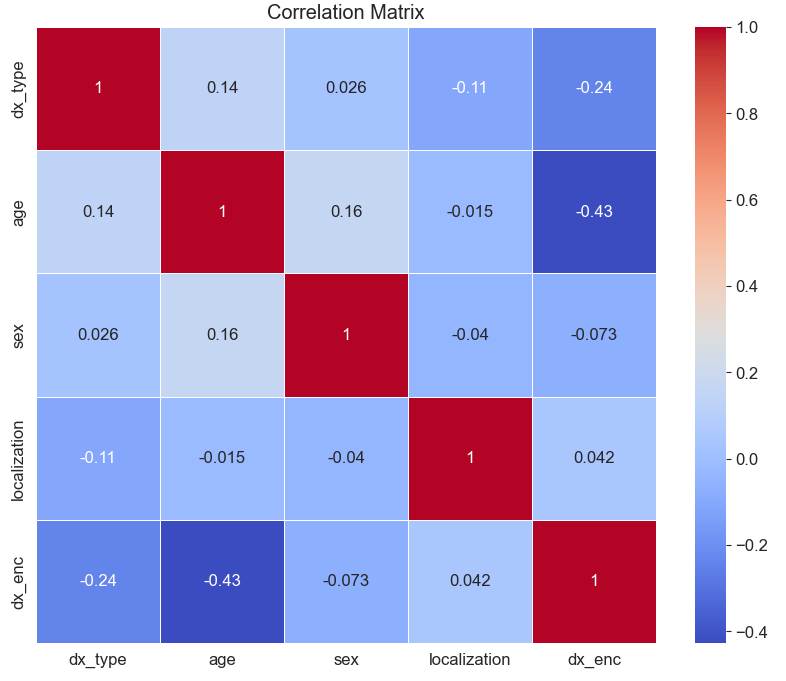
\includegraphics[width=1\linewidth]{fig5.png}
    \caption{Correlation matric between features which shows a high correlation between age and sex}
    \label{fig:fig1}
\end{figure}

Turning to the correlation matrix presented in Figure 1, the findings underscore these observations, although the matrix does not display strong correlations that would suggest any significant linear relationships between the variables of age and the categorical variables such as gender and localization. The strongest observed correlation was between age and the encoded diagnosis variable `dx-enc`, indicating that younger individuals had higher values of `dx-enc`. Despite the trends observed, the correlation coefficients are generally low, emphasizing the need for a cautious interpretation of these results and further in-depth analysis to understand the complex factors influencing the prevalence of skin cancer.


\subsection{Data Prepossessing}

\subsubsection{Data Augmentation Techniques}
To enhance the generalization capabilities of various models, we employ data augmentation. This process generates additional training samples by applying a series of transformations to the existing dataset. Common transformations include rotations, shifts in both width and height, shear mapping, zooming, horizontal and vertical flips, brightness adjustments, and nearest-neighbor pixel filling. These methods help simulate a wider range of scenarios, compensating for potential gaps in the original dataset.

\subsubsection{Learning Rate Optimization Strategies}
We implement a dynamic learning rate optimization strategy across different models. This involves a step decay schedule where the learning rate decreases periodically, allowing for more expansive steps in the initial phases and finer adjustments as the models converge. This adaptive approach is designed to improve the stability and efficacy of the training process for each model.

\subsection{Dual-Pronged Approach with Single-Input and Multi-Input CNNs for Enhanced Skin Cancer Classification}
 We have implemented two different approaches using a CNN model. The first approach utilized the sequential API from Keras. Our CNN architecture comprises a single input layer designed to handle 32x32 images with 3 channels (RGB). This is followed by two convolutional layers, the first with 32 filters of size 3x3 and the second with 64 filters. Each convolutional layer is accompanied by a ReLU activation function and a 50\% dropout layer to prevent overfitting. The final output layer is a dense layer with 7 neurons, corresponding to the number of classes, we have chosen the Softmax function as our activation function for the output layer.

A primary focus of our work was to preprocess the image data before inputting it into the model, addressing the challenge of imbalanced data. For instance, in our dataset, the Melanocytic Nevi class had 6,705 images, whereas the Dermatofibroma (df) class had only 115 images. This disparity could lead to biased predictions from our model. To counteract this, we oversampled the training dataset. Each image in X-train was transformed into a vector of length 32×32×3=3072. We randomly duplicated images from smaller classes like bcc, akiec, Vasc, and df, specifically for the training set. However, we did not modify the test set, maintaining its randomness to better evaluate how our model performs with real-life data.

The second approach involves using a multi-input layer, inspired by the notable effect of various features in the detection of different types of skin cancer. The multi-input CNN model incorporates two distinct inputs, enabling it to identify patterns and learn from multiple feature sets simultaneously. This approach draws inspiration from the work of Sánchez-Cauce, J. Pérez-Martín, and M. Luque, who developed an early prediction model for breast cancer by integrating thermal images from different perspectives with personal and clinical data [8].

In our multi-input CNN model, images are preprocessed to ensure a uniform format and scale. Continuous features are scaled appropriately, and categorical variables are one-hot encoded. The structured data inputs include sex, age, diagnosis type (dx-type), and lesion localization. The skin cancer images constitute our second input. We then combine and merge both branches to allow the model to learn simultaneously from both the structured data and the image inputs. This integrated approach aims to enhance the model's ability to make accurate predictions by leveraging the strengths of diverse data sources.
\subsection{Vision Transformer (ViT)}

Transformers, a groundbreaking architecture first introduced in the paper "Attention Is All You Need" [11], have revolutionized Natural Language Processing (NLP). These architectures, foundational to modern Large Language Models (LLMs), excel in processing sequential data due to their attention mechanisms. This attention allows dynamic focus on different parts of the input sequence, enhancing contextual understanding. In computer vision, however, Convolutional Neural Networks (CNNs) have traditionally dominated, primarily due to their ability to process pixel data and capture spatial hierarchies in images [11]. Yet, the recent adaptation of Transformer architectures to computer vision tasks has opened new avenues. The Vision Transformer (ViT), particularly in its "ViT-Base-Patch16-224" variant from Google's collection on Hugging Face, represents a paradigm shift from CNNs [12]. This model, optimized for image classification, processes images by dividing them into 16x16 pixel patches and applying self-attention across these patches, a method akin to processing word embeddings in NLP.

\subsubsection{Application in Skin Cancer Detection}
In our skin cancer detection project, we leverage the "ViT-Base-Patch16-224" model's unique capabilities. Its attention mechanism can focus on relevant image patches, such as areas with lesions, aiding in distinguishing between benign and malignant skin conditions. This precision is invaluable in medical imaging, where diagnostic accuracy can significantly impact patient treatment and outcomes.

\subsubsection{Data Augmentation for Enhanced Generalization}
Given the Vision Transformer's requirement for substantial data to generalize effectively, we employ data augmentation techniques to enhance our dataset. Data augmentation involves artificially expanding the dataset by applying various transformations to the images, such as rotation, scaling, and color adjustments. This process not only increases the quantity of training data but also introduces variability, helping the model to learn more robust features and reduce overfitting. Such augmentation is crucial for achieving high accuracy, especially when dealing with complex medical images where subtle differences can be critical.

The use of the "ViT-Base-Patch16-224" model, combined with data augmentation, presents a novel approach in computer vision. This method's adaptability and effectiveness in image classification tasks make it a powerful tool for applications like skin cancer detection, where detailed and accurate image analysis is essential.

\subsection{Deep Residual Learning Framework for ResNet-101}

In line with the advancements detailed by He et al. (2015)[13], our approach involves the implementation of the ResNet-101 architecture within the deep residual learning framework. This framework is pivotal for training deeper networks by reformulating layer functions to learn residual mappings, which significantly eases the optimization process and facilitates the construction of deeper network architectures with improved accuracy.

\subsubsection{ResNet-101 Architecture}

The ResNet-101 model exemplifies a deeper architecture that extends the principles of residual learning. It is composed of multiple residual blocks, each designed with a specific formula to facilitate learning of complex patterns. The typical structure of a residual block in ResNet-101 can be expressed as:

\begin{equation}
    y = F(x, \{W_i\}) + x
\end{equation}

In this equation, \( y \) represents the output of the residual block, and \( x \) denotes the input to that block. The function \( F(x, \{W_i\}) \) is the residual function, which is the core component of the block. Here, \( \{W_i\} \) symbolizes the set of weights associated with the block. The residual function \( F \) is designed to learn the residual mapping, or the difference between the input and the target output [11].

The addition of \( x \) to the output of the function \( F \) is a crucial aspect of the ResNet architecture, known as the shortcut connection. This connection enables the network to learn identity mappings by default, simplifying the learning process and allowing for deeper network architectures without a significant increase in computational complexity. These shortcut connections facilitate the flow of gradients during training, which helps in mitigating the vanishing gradient problem common in deep networks.


\subsubsection{Customization and Evaluation for Skin Cancer Dataset}

Adapting the ResNet-101 architecture for skin cancer detection involves customizing the network to handle the unique characteristics of dermatological imaging. The model will be fine-tuned and evaluated on a dedicated skin cancer dataset, ensuring that the deep learning approach is well-suited for accurate detection and classification of various skin cancer types [14].

\section{Evaluation Metrics}

To effectively evaluate the performance of our model in classifying each class, we employed several widely recognized metrics in the field of machine learning. These metrics provide a comprehensive understanding of the model's accuracy, precision, recall, and overall predictive performance.

\subsection{Precision}
Precision measures the accuracy of positive predictions. It is defined as the ratio of true positives (TP) to the sum of true positives and false positives (FP). High precision indicates that the model is reliable in its positive classifications.

\textbf{Precision Formula:}
\begin{equation}
    \text{Precision} = \frac{TP}{TP + FP}
\end{equation}

\subsection{Recall}
Recall, also known as sensitivity, measures the model’s ability to correctly identify actual positives. It is the ratio of true positives to the sum of true positives and false negatives (FN). High recall indicates that the model is effective in identifying most positive cases.

\textbf{Recall Formula:}
\begin{equation}
    \text{Recall} = \frac{TP}{TP + FN}
\end{equation}

\subsection{F1 Score}
The F1 Score is the harmonic mean of precision and recall. It is particularly useful when the class distribution is imbalanced. The F1 Score provides a balance between precision and recall, giving a single metric to assess the model's accuracy.

\textbf{F1 Score Formula:}
\begin{equation}
    \text{F1 Score} = 2 \times \frac{\text{Precision} \times \text{Recall}}{\text{Precision} + \text{Recall}}
\end{equation}

\subsection{Performance Analysis}
In our model evaluation, we focused on the F1 Score, precision, recall, and the confusion matrix for each class. Notably, class five exhibited the highest precision and recall values, indicating a high degree of accuracy in classifying this particular class. The confusion matrix reinforced this finding, displaying the largest number of true positive predictions at 1083 for class five. Overall, the confusion matrix demonstrated a satisfactory performance of the model across our dataset.

\section{Performance Evaluation and Results}

\subsection{CNN Model Performance}

The initial implementation of our Convolutional Neural Network (CNN) model yielded an accuracy of 71\%, which is commendable for image classification tasks, especially considering challenges such as low image quality, varied lighting conditions, and constraints related to image size and computational resources. To enhance the model's predictive capability, we integrated additional label features, recognizing their significant correlation with the target variable. This led to the development of a multi-input CNN model capable of processing both images and other feature types (such as location, age, and sex) to predict skin cancer types. This modification resulted in a notable increase in accuracy, reaching up to 77\%, making it our most effective model for this dataset.

By integrating additional features, such as age and location, into a multi-input CNN, accuracy improved significantly to 81\%. This method yielded a robust model that predicts skin cancer types more accurately by considering both image and non-image data.

Prior to balancing the dataset, our model's accuracy was at 65\% with a tendency to overfit—training accuracy was 90\% compared to 65\% for testing. After introducing data augmentation and oversampling, we managed to minimize overfitting and increase testing accuracy to nearly 71\%. The model performed best with a batch size of 34 over 150 epochs.
\begin{figure}[h]
    \centering
    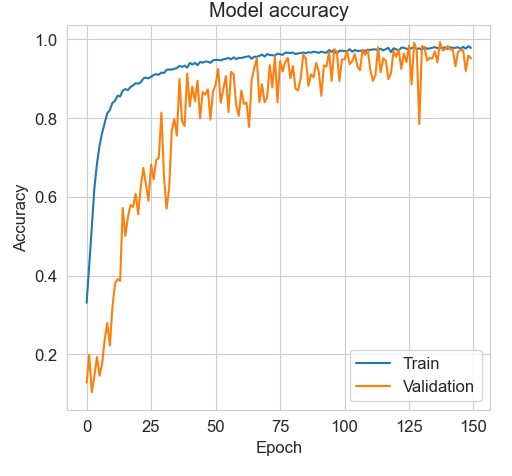
\includegraphics[width=1\linewidth]{fig6.png}
    \caption{Evolution of CNN model accuracy across 150 training epochs.}
    \label{fig:fig1}
\end{figure}

\subsection{ResNet-101 Performance}

The implementation of the ResNet-101 model demonstrated substantial improvement over the course of training. Initially, the model started with an accuracy of approximately 68.89\% in the first epoch, gradually increasing to 89.28\% by the 20th epoch. The validation accuracy paralleled this trend, starting at 68.95\% and reaching up to 80.48\%. This progression signifies the model's capacity to learn effectively and adapt to the intricacies of skin cancer detection. The detailed training and validation accuracies per epoch are visually represented (Figure \ref{fig:model-accuracies}), showcasing the comparative performance of the ResNet-101 model across 20 epochs.

\subsection{Vision Transformer (ViT) Performance}

The Vision Transformer (ViT) model also showed a promising trend in performance. Starting with a training accuracy of 66.48\% in the first epoch, it exhibited a consistent increase, achieving 72.46\% accuracy by the 20th epoch. The validation accuracy observed a similar pattern, beginning at 61.86\% and culminating at 73.04\%. These results indicate that the ViT model, while exhibiting some fluctuations, also holds potential in the domain of skin cancer classification, as reflected in the training and validation accuracies over the training period.

\subsection{Comparative Analysis}

The comparative analysis of the CNN, ResNet-101, and ViT models, as illustrated in the graph, provides valuable insights into their respective learning curves and generalization capabilities. The ResNet-101 model, in particular, displayed a notable balance between learning efficiency and validation performance, suggesting its suitability for complex tasks like skin cancer detection. The enhanced accuracy achieved by incorporating additional features in the CNN model also highlights the importance of leveraging diverse data inputs for improved diagnostic predictions.

The following graph (Figure \ref{fig:model-accuracies}) illustrates the training and validation accuracies of the ResNet-101 and ViT models over 20 epochs. In this graph, the ResNet-101 model's training accuracy is represented by a dark blue line with circular markers, while its validation accuracy is shown in light blue with square markers. Similarly, for the ViT model, the training accuracy is depicted in dark green with triangular markers, and the validation accuracy is in light green with 'x' markers.

\begin{figure}[h]
    \centering
    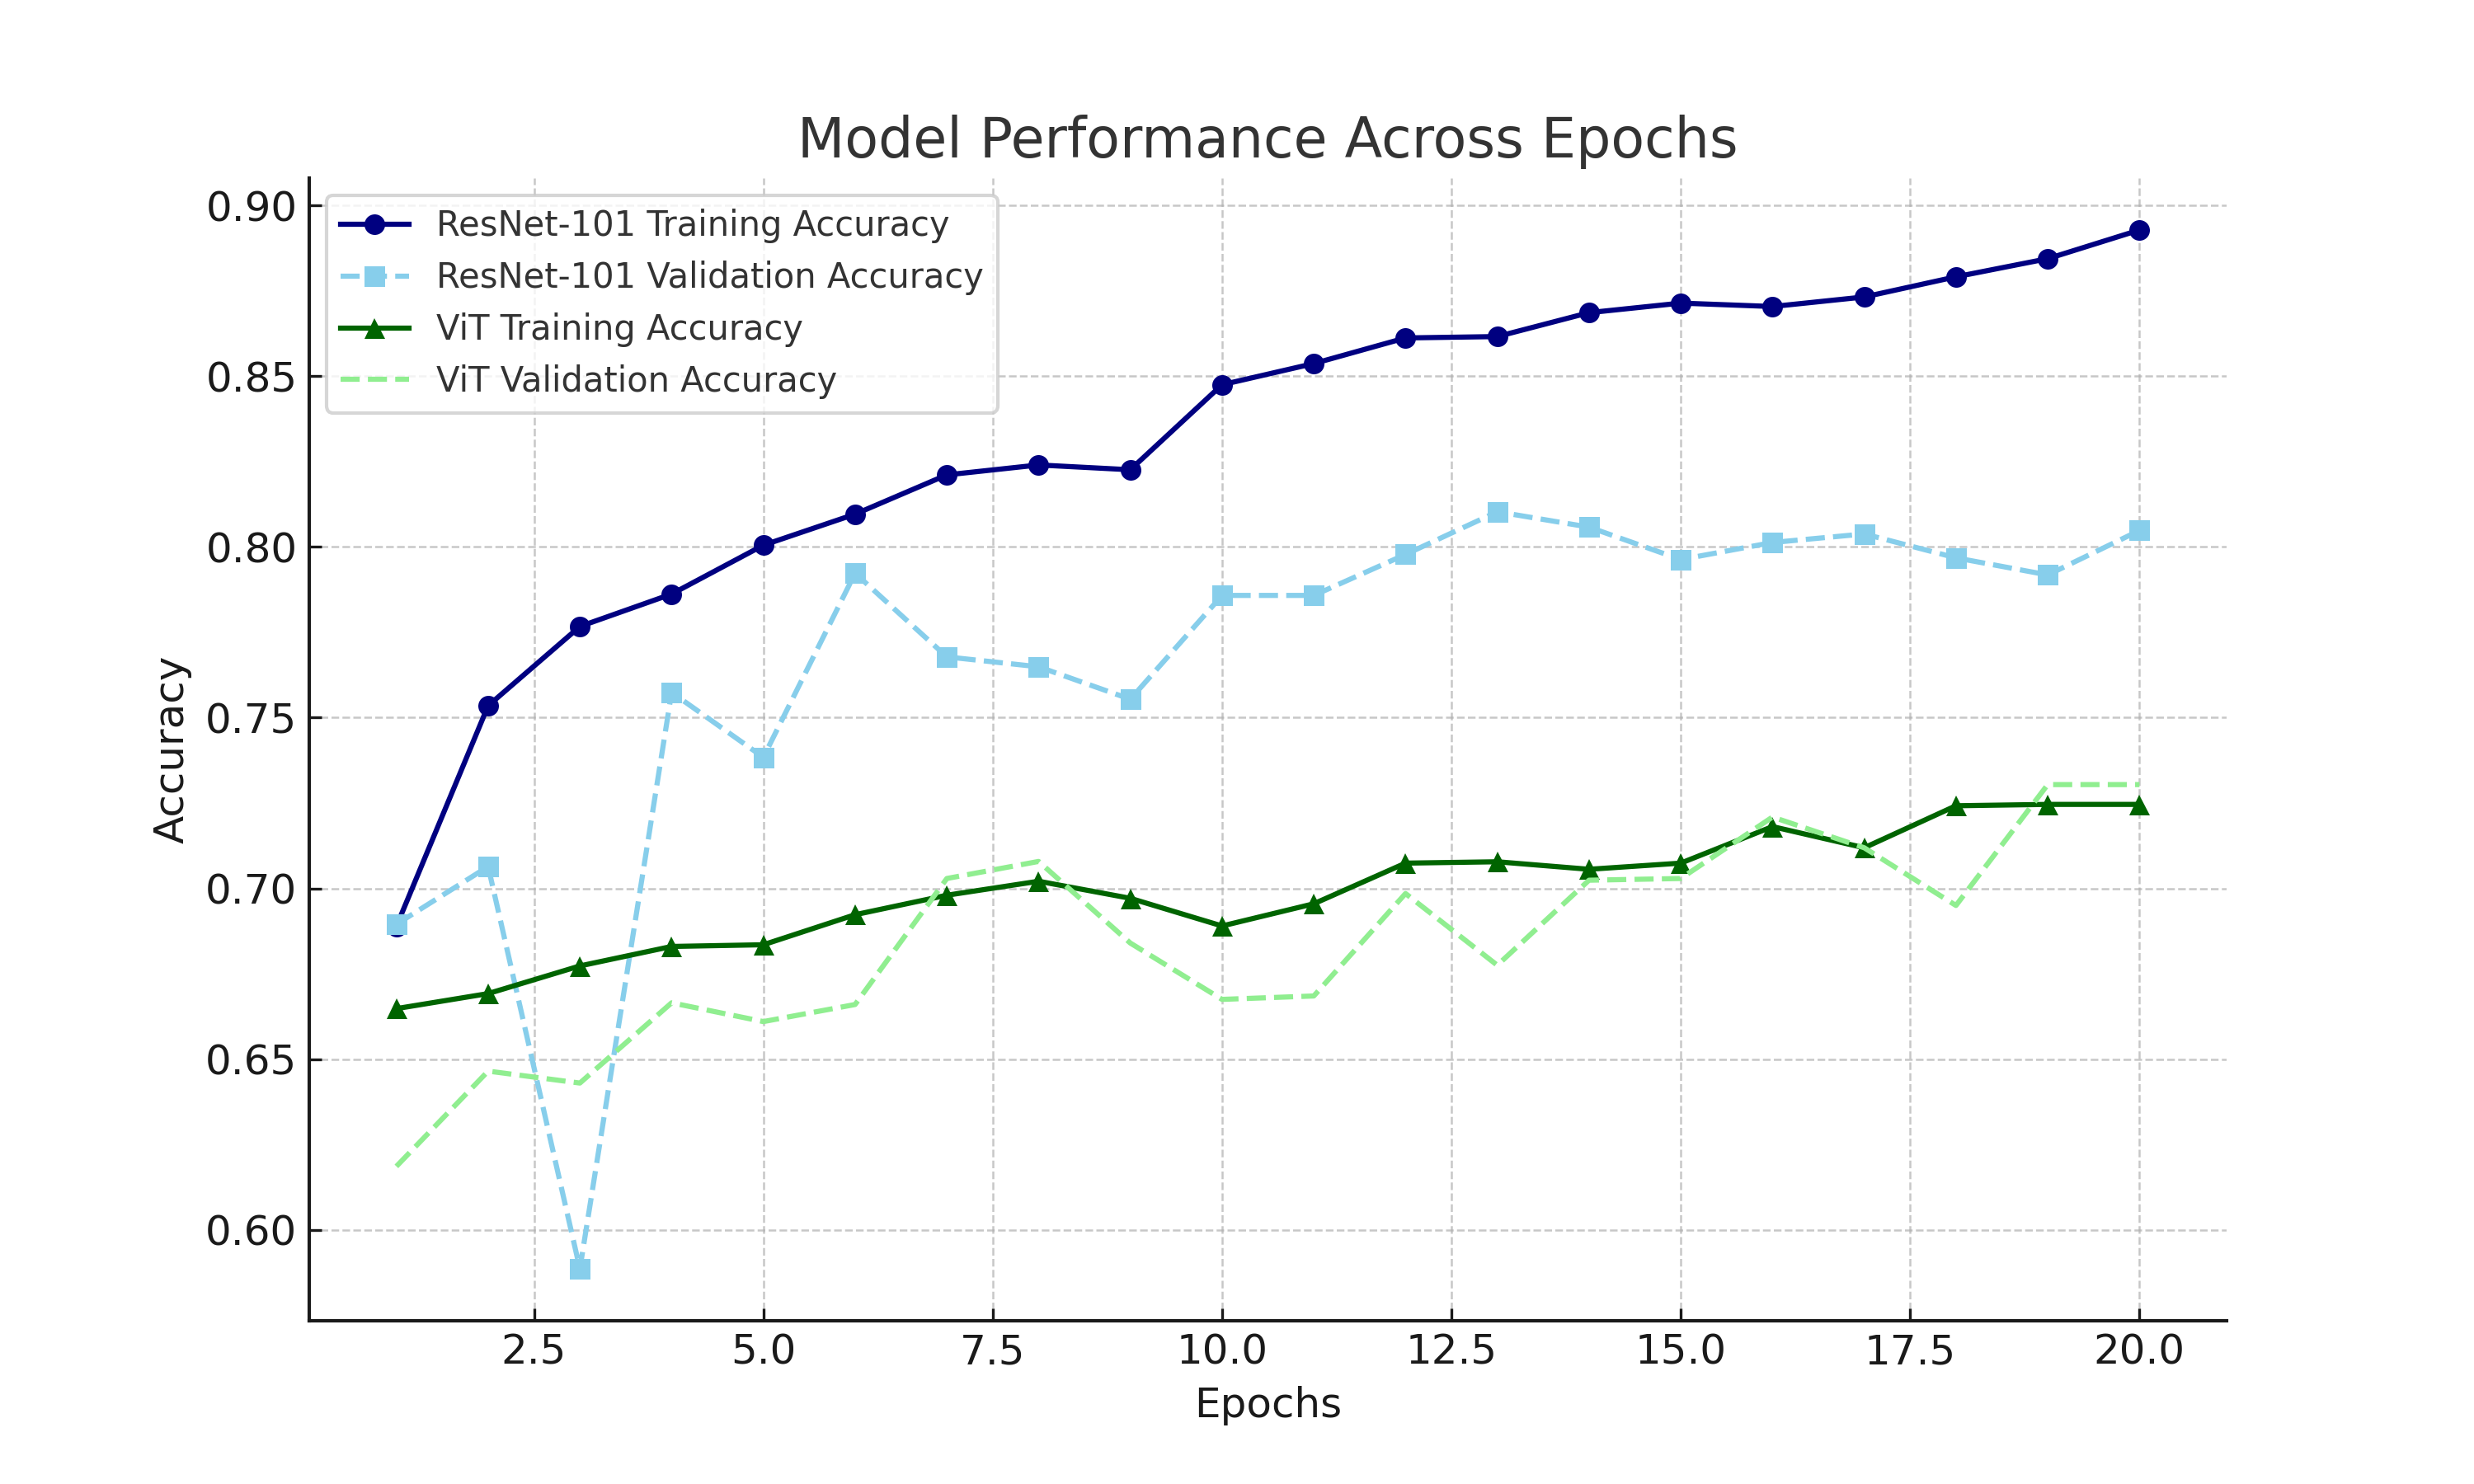
\includegraphics[width=1.05\linewidth]{fig4.png}
    \caption{Training and validation accuracies of ResNet-101 and ViT models over 20 epochs.}
    \label{fig:model-accuracies}
\end{figure}


In conclusion, the results from these models underscore the potential of deep learning approaches in medical image analysis, especially for challenging tasks such as accurate skin cancer classification.


\section{Conclusion and Future Scope}
After evaluating the performance of different models for skin cancer classification, it's evident that each approach has its merits. While the initial CNN model performed reasonably well at 71\% accuracy, the integration of additional label features significantly boosted its predictive power, achieving a commendable 81\% accuracy. However, the ResNet-101 model showcased remarkable learning capabilities, steadily progressing from 68.89\% to an impressive 89.28\% accuracy over 20 epochs, outperforming other models in terms of final accuracy. The Vision Transformer (ViT) also displayed promise, showing consistent improvement and reaching 73.04\% accuracy. Overall, while the multi-input CNN excelled after feature enhancement, the ResNet-101 model emerged as the frontrunner, demonstrating exceptional adaptability and performance in skin cancer detection throughout its training.

\section*{Acknowledgment}

The authors would like to express their gratitude to Dr. Sukhchandan, the course instructor of CSCI 4155 at Dalhousie University, for her invaluable guidance throughout this project. Special thanks to the teaching assistant, Ashutosh Sagar for his consistent support and assistance. We also acknowledge the use of OpenAI's ChatGPT for assistance in aspects of formatting and content refinement. It's important to clarify that the substantive research, analysis, and conclusions presented in this paper are solely the work of the authors. Tools like ChatGPT were used judiciously to enhance the presentation and structure of the paper, ensuring a clear and coherent narrative


\begin{thebibliography}{00}
\bibitem{b1} Dildar, M.; Akram, S.; Irfan, M.; Khan, H.U.; Ramzan, M.; Mahmood, A.R.; Alsaiari, S.A.; Saeed, A.H.M; Alraddadi, M.O.; Mahnashi, M.H. Skin Cancer Detection: A Review Using Deep Learning Techniques. Int. J. Environ. Res. Public Health 2021, 18, 5479. https://doi.org/10.3390/ijerph18105479
\bibitem{b2} Noel Codella, Veronica Rotemberg, Philipp Tschandl, M. Emre Celebi, Stephen Dusza, David Gutman, Brian Helba, Aadi Kalloo, Konstantinos Liopyris, Michael Marchetti, Harald Kittler, Allan Halpern: "Skin Lesion Analysis Toward Melanoma Detection 2018: A Challenge Hosted by the International Skin Imaging Collaboration (ISIC)", 2018; https://arxiv.org/abs/1902.03368
\bibitem{b3} Dosovitskiy, A.; Beyer, L.; Kolesnikov, A.; Weissenborn, D.; Zhai, X.; Unterthiner, T.; Dehghani, M.; Minderer, M.; Heigold, G.; Gelly, S.; Uszkoreit, J.; Houlsby, N. "An Image is Worth 16x16 Words: Transformers for Image Recognition at Scale", 2021; arXiv preprint arXiv:2010.11929.
\bibitem{b4} U. Vaze, S. Palekar, and A. Galagali, “SKIN CANCER DETECTION AND CLASSIFICATION USING MACHINE LEARNING TECHNIQUES SKIN CANCER DETECTION AND CLASSIFICATION USING MACHINE LEARNING TECHNIQUES.”. Goa University, 2020/2021. Available: http://iqac.unigoa.ac.in/criterion1/1.3.4-ELO-01.pdf.
\bibitem{b5} Kumar, R. Senthil, Amarjeet Singh, Sparsha Srinath, Nimal Kurien Thomas, and Vishal Arasu. “Skin Cancer Detection Using Deep Learning.” In 2022 International Conference on Electronics and Renewable Systems (ICEARS), 1724–1730. IEEE, 2022.
\bibitem{b6} S. Mst, Akter, H. Shahriar, S. Sneha, and A. Cuzzocrea, “Multi-class Skin Cancer Classification Architecture Based on Deep Convolutional Neural Network.” Accessed: May 09, 2023. [Online]. Available: https://arxiv.org/ftp/arxiv/papers/2303/2303.07520.pdf
\bibitem{b7} A. S. Qureshi and T. Roos, “Transfer Learning with Ensembles of Deep Neural Networks for Skin Cancer Detection in Imbalanced Data Sets,” arXiv.org, May 17, 2021. https://arxiv.org/abs/2103.12068 (accessed Dec. 06, 2023)
\bibitem{b8} R. Sánchez-Cauce, J. Pérez-Martín, and M. Luque, “Multi-input convolutional neural network for breast cancer detection using thermal images and clinical data,” Computer Methods and Programs in Biomedicine, vol. 204, p. 106045, Jun. 2021, doi: https://doi.org/10.1016/j.cmpb.2021.106045.
\bibitem{b9} C. Subakan, M. Ravanelli, S. Cornell, M. Bronzi and J. Zhong, "Attention Is All You Need In Speech Separation," ICASSP 2021 - 2021 IEEE International Conference on Acoustics, Speech and Signal Processing (ICASSP), Toronto, ON, Canada, 2021, pp. 21-25, doi: 10.1109/ICASSP39728.2021.9413901.
\bibitem{b10} A. Dosovitskiy et al., "An Image is Worth 16x16 Words: Transformers for Image Recognition at Scale," in International Conference on Learning Representations (ICLR), 2021.
\bibitem{b11} Hugging Face, ``Vision Transformer (ViT) documentation,'' 2023. Available: https://huggingface.co/docs/transformers/model\textunderscore doc/vit. 
\bibitem{b12} He, Kaiming, Xiangyu Zhang, Shaoqing Ren, and Jian Sun. "Deep residual learning for image recognition." In Proceedings of the IEEE conference on computer vision and pattern recognition, pp. 770-778. 2016.
\bibitem{13} He, Kaiming, Xiangyu Zhang, Shaoqing Ren, and Jian Sun. "Deep residual learning for image recognition." In Proceedings of the IEEE conference on computer vision and pattern recognition, pp. 770-778. 2016.
\bibitem{14} Microsoft, “ResNet-101,” Hugging Face, [Online]. Available: https://huggingface.co/microsoft/resnet-101. [Accessed: 10-10-2023].
\end{thebibliography}
\vspace{12pt}


\end{document}
